\documentclass[aspectratio=169,12pt]{beamer}
\usepackage[utf8]{inputenc}
\usepackage{amsmath, amssymb}
\usepackage{booktabs}
\usepackage{xcolor}
\usepackage{colortbl}
\usepackage{hyperref}
\usepackage{makecell}
\usepackage{ragged2e}
\usepackage{bytefield}
\usepackage{tikz}
\usetikzlibrary{arrows.meta, positioning, shapes.geometric, calc, tikzmark, shapes.misc}
\usepackage{tcolorbox}
\usetheme{Madrid}

\definecolor{cachecolor}{RGB}{200,220,255}
\definecolor{memcolor}{RGB}{255,220,200}
\definecolor{modifiedcolor}{RGB}{255,200,200}
\definecolor{exclusivecolor}{RGB}{200,255,200}
\definecolor{messageblue}{RGB}{70,130,255}
\definecolor{timecolor}{RGB}{200,100,0}
\definecolor{stateM}{RGB}{255,200,200}
\definecolor{stateE}{RGB}{200,255,200}
\definecolor{stateS}{RGB}{200,200,255}

\title{MESI Protocol}
\subtitle{Computer Architecture}
\author{Course 234267}
\date{}
\begin{document}
\frame{\titlepage}

%==========================================
\begin{frame}{Multi-processor System}
\begin{block}{Memory System Coherence}
A memory system is coherent if:
\end{block}

\begin{enumerate}
\item If P1 writes to address X, and later on, P2 reads X, and there are no other writes to X in between
    \begin{itemize}
    \item[$\Rightarrow$] P2's read returns the value written by P1's write
    \end{itemize}
\item Writes to the same location are serialized:
    \begin{itemize}
    \item Two writes to location X are seen in the same order by all processors
    \end{itemize}
\end{enumerate}

\vspace{1em}
\begin{center}
% Placeholder for processor-cache-memory diagram
\framebox[0.6\textwidth][c]{
\parbox{0.55\textwidth}{\centering
[Diagram: Two processors with L1 caches\\
connected to shared L2 cache and memory]
}}
\end{center}
\end{frame}

%==========================================
\begin{frame}{MESI Protocol States}
Each cache line can be in one of 4 states:

\begin{itemize}
\item \textbf{Invalid (I)} -- Line's data is not valid
\vspace{0.5em}
\item \textbf{Shared (S)} -- Line is valid and not dirty, copies may exist in other processors
\vspace{0.5em}
\item \textbf{Exclusive (E)} -- Line is valid and not dirty, other processors do not have the line in their local caches
\vspace{0.5em}
\item \textbf{Modified (M)} -- Line is valid and dirty, other processors do not have the line in their local caches
\end{itemize}
\end{frame}

%==========================================
\begin{frame}{Multi-processor System: Example (1/3)}
\begin{columns}
\column{0.5\textwidth}
\textbf{Sequence of operations:}
\begin{itemize}
\item P1 reads 1000
\item P1 writes 1000
\end{itemize}

\vspace{1em}
\textbf{Initial state:}
\begin{itemize}
\item Memory[1000]: 5
\item Both caches empty
\end{itemize}

\column{0.5\textwidth}
\begin{center}
% Placeholder for state diagram
\framebox[0.9\columnwidth][c]{
\parbox{0.85\columnwidth}{\centering
[Diagram: P1 cache transitions\\
from Invalid $\rightarrow$ Exclusive $\rightarrow$ Modified\\
P1 L1: [1000]: 6 (M)\\
P2 L1: Invalid\\
L2: [1000]: 5, CVB: 001]
}}
\end{center}
\end{columns}
\end{frame}

%==========================================
\begin{frame}{Multi-processor System: Example (2/3)}
\begin{columns}
\column{0.5\textwidth}
\textbf{Continuing sequence:}
\begin{itemize}
\item P2 reads 1000
\item L2 snoops 1000
\item P1 writes back 1000
\item P2 gets 1000
\end{itemize}

\vspace{1em}
\textbf{Result:}
\begin{itemize}
\item Both P1 and P2 have line in Shared state
\item Value = 6
\end{itemize}

\column{0.5\textwidth}
\begin{center}
% Placeholder for state diagram
\framebox[0.9\columnwidth][c]{
\parbox{0.85\columnwidth}{\centering
[Diagram: State transitions\\
P1: M $\rightarrow$ S\\
P2: I $\rightarrow$ S\\
Both caches: [1000]: 6 (S)\\
L2: [1000]: 6, CVB: 101]
}}
\end{center}
\end{columns}
\end{frame}

%==========================================
\begin{frame}{Multi-processor System: Example (3/3)}
\begin{columns}
\column{0.5\textwidth}
\textbf{Final operation:}
\begin{itemize}
\item P2 requests for ownership with write intent
\end{itemize}

\vspace{1em}
\textbf{Result:}
\begin{itemize}
\item P1: Invalid
\item P2: Exclusive (then can modify)
\end{itemize}

\column{0.5\textwidth}
\begin{center}
% Placeholder for state diagram
\framebox[0.9\columnwidth][c]{
\parbox{0.85\columnwidth}{\centering
[Diagram: State transitions\\
P1: S $\rightarrow$ I\\
P2: S $\rightarrow$ E\\
P1 L1: Invalid\\
P2 L1: [1000]: 6 (E)\\
L2: CVB: 01]
}}
\end{center}
\end{columns}
\end{frame}

%==========================================
\begin{frame}{Core Valid Bits (CVB)}
\begin{block}{What are Core Valid Bits?}
L2 keeps track of the presence of each line in each Core's L1 caches using a bit vector
\end{block}

\vspace{0.5em}
\textbf{Purpose:}
\begin{itemize}
\item Determine if it needs to send a snoop to a processor
\item Determine in what state to provide a requested line (S or E)
\item Track which cores have copies of each cache line
\end{itemize}

\vspace{0.5em}
\textbf{Implementation:}
\begin{itemize}
\item One bit per core for each L2 cache line
\item Bit = 1: Core may have the line in its L1 cache
\item Bit = 0: Core does not have the line in its L1 cache
\end{itemize}

\vspace{0.5em}
\textbf{Example:}
\begin{itemize}
\item CVB = 001: Only Core 0 has the line
\item CVB = 110: Cores 1 and 2 have the line
\item CVB = 000: No core has the line
\end{itemize}
\end{frame}

%==========================================
\begin{frame}{Inclusion Property}
\begin{alertblock}{L2 Cache Inclusion}
The L2 cache must guarantee that all L1 cache lines are included in L2
\end{alertblock}

\vspace{0.5em}
\textbf{Why Inclusion Matters:}
\begin{itemize}
\item Simplifies coherence protocol
\item L2 can track all L1 contents
\item Enables efficient snooping decisions
\end{itemize}

\vspace{0.5em}
\textbf{When L2 Evicts a Line:}
\begin{itemize}
\item L2 must first invalidate the line in all L1 caches
\item L2 sends snoop invalidate to all processors with CVB bit set
\item If line is Modified in L1:
    \begin{itemize}
    \item L1 responds with updated data
    \item L2 writes updated value to memory during eviction
    \end{itemize}
\end{itemize}

\vspace{0.5em}
\textbf{Maintaining Inclusion:}
\begin{itemize}
\item L2 capacity must be larger than sum of L1 caches
\item L2 eviction triggers L1 invalidation
\item Ensures coherence is maintained at L2 level
\end{itemize}
\end{frame}

%==========================================
\begin{frame}{MESI Protocol States - Summary}
\begin{table}[h]
\centering
\begin{tabular}{|c|c|c|c|}
\hline
\rowcolor{blue!20}
\textbf{State} & \textbf{Valid} & \textbf{Modified} & \textbf{Copies may exist} \\
& & & \textbf{in other processors} \\
\hline
Invalid & No & N.A. & N.A. \\
\hline
Shared & Yes & No & Yes \\
\hline
Exclusive & Yes & No & No \\
\hline
Modified & Yes & Yes & No \\
\hline
\end{tabular}
\end{table}

\vspace{1em}
\begin{block}{Important Rule}
A modified line must be exclusive
\begin{itemize}
\item Otherwise, another processor with the line will be using stale data
\item Therefore, before modifying a line, a processor must request ownership
\end{itemize}
\end{block}
\end{frame}

%==========================================
\begin{frame}{MESI Protocol Example - 4 Processors}
\small
Four-processor shared-memory system with MESI protocol

\begin{table}[h]
\centering
\begin{tabular}{|l|c|c|c|c|c|}
\hline
\rowcolor{blue!20}
\textbf{Operation} & \textbf{P0} & \textbf{P1} & \textbf{P2} & \textbf{P3} & \textbf{CVBs} \\
\hline
Initial State & I & I & I & I & 0000 \\
\hline
P0 reads X & E & I & I & I & 1000 \\
\hline
P1 reads X & S & S & I & I & 1100 \\
\hline
P2 reads X & S & S & S & I & 1110 \\
\hline
P3 writes X & I & I & I & M & 0001 \\
\hline
P0 reads X & S & I & I & S & 1001 \\
\hline
\end{tabular}
\end{table}

\textbf{Key observations:}
\begin{itemize}
\item First reader gets Exclusive state (if no other copies exist)
\item Write operation invalidates all other copies
\item Subsequent reads after a write result in Shared state
\end{itemize}
\end{frame}

%==========================================
\begin{frame}{MESI Question 2 - Setup}
\textbf{System Configuration:}
\begin{itemize}
\item 3 Core processor with MESI
\item Each core has an L1 cache, L2 cache is shared
\end{itemize}

\textbf{Message Types:}
\begin{columns}
\column{0.5\textwidth}
\textbf{L1 $\rightarrow$ L2:}
\begin{itemize}
\item Read Address (A)
\item RFO (A) - Request for Ownership
\item Data (A)
\end{itemize}

\column{0.5\textwidth}
\textbf{L2 $\rightarrow$ L1/Memory:}
\begin{itemize}
\item Read Address (A) to memory
\item Data (A) to L1 with MESI state
\item RFO (A) - after RFO from L1
\item Snoop (A) to L1
\end{itemize}
\end{columns}

\vspace{1em}
\textbf{Timing:}
\begin{itemize}
\item L1 $\leftrightarrow$ L2: 10ns
\item L2 $\leftrightarrow$ Memory: 100ns
\end{itemize}
\end{frame}

%==========================================
\begin{frame}{MESI Question 2 - Solution}
\tiny
\begin{table}[h]
\centering
\begin{tabular}{|p{1.5cm}|c|c|c|c|c|c|c|p{5cm}|}
\hline
\rowcolor{blue!20}
\textbf{Operation} & \textbf{P1} & \textbf{P2} & \textbf{P3} & \multicolumn{3}{c|}{\textbf{CVBs}} & \textbf{Time} & \textbf{Messages} \\
\cline{5-7}
& & & & P1 & P2 & P3 & & \\
\hline
Initial & I & I & I & 0 & 0 & 0 & 0 & - \\
\hline
P2 reads A & I & E & I & 0 & 1 & 0 & 220 & L1 miss/req to L2, L2 Miss/req to Mem, Mem data to L2, L2 data to L1 \\
\hline
P2 writes A & I & M & I & 0 & 1 & 0 & 0 & No messages (local operation) \\
\hline
P1 reads A & S & S & I & 1 & 1 & 0 & 40 & P1: miss/req to L2, P2: L2→L1 snoop, P2: L1 to L2 data, P1: L2 to L1 data \\
\hline
P2 reads A & S & S & I & 1 & 1 & 0 & 0 & Hit in cache \\
\hline
P3 reads A & S & S & S & 1 & 1 & 1 & 20 & P3: L1 miss/Req to L2, L2 to P3 data \\
\hline
P3 writes A & I & I & M & 0 & 0 & 1 & 30 & P3: L1 to L2 RFO, L2 snoop P1+P2, L2 to P3 RFO granted \\
\hline
\end{tabular}
\end{table}
\normalsize
\end{frame}

%==========================================
\begin{frame}{Read For Ownership (RFO)}
\begin{block}{RFO Request}
A signal from private to shared cache (L1$\rightarrow$L2) requesting cache line exclusivity for write intent
\end{block}

\textbf{RFO Process:}
\begin{enumerate}
\item L1 sends RFO to L2/LLC
\item MLC/LLC invalidates cache line in other L1s
\item MLC/LLC responds to L1 that RFO has been granted
\item L1 can now modify cache line
\end{enumerate}

\vspace{1em}
\begin{alertblock}{Key Point}
RFO ensures exclusive access before modification, maintaining cache coherence
\end{alertblock}
\end{frame}

%==========================================
\begin{frame}{Global Observation (GO)}
\begin{block}{Global Observation}
L2 sends a notification to all processors before delivering the actual data to the requesting L1 cache. This notification informs all processors that a specific cache line is being accessed.
\end{block}

\textbf{The Global Observation message indicates the MESI state (E or S) for the requested line}

\vspace{1em}
\textbf{Two-step L1$\rightarrow$L2 line request:}
\begin{enumerate}
\item \textbf{GO} - Global Observation with MESI state
\item \textbf{Fill} - Actual data transfer
\end{enumerate}

\vspace{1em}
\begin{alertblock}{Note}
GO and data may be sent at different cycles:
\begin{itemize}
\item GO is the outcome of a tag-hit
\item Data comes from the data array
\end{itemize}
\end{alertblock}
\end{frame}

%==========================================
\begin{frame}{MESI Question 3 - Exam Problem Setup}
\footnotesize
\textbf{System Configuration:}
\begin{itemize}
\item 2 processors (P0 and P1) with MESI protocol
\item Each processor has L1 cache, shared L2 cache (inclusive)
\item Direct-mapped caches with write allocate + write back
\end{itemize}

\textbf{Latencies:}
\begin{itemize}
\item L1 access: 3ns
\item L1 $\leftrightarrow$ L2 message: 20ns
\item L2 $\leftrightarrow$ Memory message: 90ns
\end{itemize}

\textbf{Important Details:}
\begin{itemize}
\item Parallel messages possible on different channels
\item X1-X5 are separate cache lines
\item X1-X4 map to same L1 set, X5 to different L1 set
\item X1-X2 map to same L2 set, X3-X5 to different L2 set
\end{itemize}
\end{frame}

\begin{frame}{MESI Question 3 - Solution}
\tiny
\vspace{-0.5cm}
\begin{columns}[t]
\column{0.5\textwidth}
\textbf{System:} 2 proc, MESI, L1 priv, L2 shared incl, direct-map\\
\textbf{Latencies:} L1: 3ns, L1$\leftrightarrow$L2: 20ns, L2$\leftrightarrow$Mem: 90ns
\column{0.5\textwidth}
\textbf{L1 Mapping:} X1,X2,X3,X4 → same set; X5 → different set\\
\textbf{L2 Mapping:} X1,X2 → same set; X3,X4,X5 → different set
\end{columns}

\vspace{0.1cm}
\begin{table}[h]
\centering
\renewcommand{\arraystretch}{0.8}
\resizebox{\textwidth}{!}{%
\begin{tabular}{|c|l|l|c|c|c|c|}
\hline
\rowcolor{gray!20}
\# & \textbf{Op} & \textbf{Messages Sent} & \textbf{Time} & \multicolumn{2}{c|}{\textbf{CVB}} & \textbf{State} \\
\cline{5-6}
\rowcolor{gray!20}
 & & & (ns) & P0 & P1 & \\
\hline
\only<2->{1} & \only<2->{P0 reads X1} & 
\only<2->{\textcolor{messageblue}{P0→L1 miss, P0-L1→L2 read miss, L2→MEM read, MEM→L2 data, L2→P0-L1 data, P0→data}} & 
\only<2->{\textcolor{timecolor}{226}} & 
\only<2->{1} & 
\only<2->{0} & 
\only<2->{\cellcolor{stateE}E} \\
\hline
2 & P1 writes X3 & 
P1→L1 miss, P1-L1→L2 read miss, L2→MEM read, MEM→L2 data, L2→P1-L1 data, P1 write & 
226 & 
0 & 
1 & 
\cellcolor{stateM}M \\
\hline

3 & P1 writes X4 & 
\only<2->{\textcolor{messageblue}{P1→L1 miss, \underline{P1-L1→L2 wr X3}, P1-L1→L2 rd miss, \underline{L2→MEM wr}, L2→MEM rd, MEM→L2, L2→P1-L1, P1 wr}} & 
\only<2->{\textcolor{timecolor}{336}} & 
\only<2->{0} & 
\only<2->{1} & 
\only<2->{\cellcolor{stateM}M} \\
\hline
4 & P1 writes X5 & 
\only<2->{\textcolor{messageblue}{P1→L1 miss, P1-L1→L2 rd miss, \underline{L2→P1 snoop X4}, \underline{P1→L2 data}, \underline{L2→MEM wr}, L2→MEM rd, MEM→L2, L2→P1, P1 wr}} & 
\only<2->{\textcolor{timecolor}{356}} & 
\only<2->{0} & 
\only<2->{1} & 
\only<2->{\cellcolor{stateM}M} \\
\hline
5 & P0 reads X5 & 
\only<2->{\textcolor{messageblue}{P0→L1 miss, P0-L1→L2 rd miss, \textbf{L2→P1 snoop}, \textbf{P1→L2 data}, L2→P0 data, P0 read}} & 
\only<2->{\textcolor{timecolor}{86}} & 
\only<2->{1} & 
\only<2->{1} & 
\only<2->{\cellcolor{stateS}S} \\
\hline
6 & P1 reads X4 & 
\only<2->{\textcolor{messageblue}{P1→L1 miss, P1-L1→L2 rd miss, \{L2→P1+P0 snoop, L2→MEM wr X5\}, L2→MEM rd, MEM→L2, L2→P1, P1 rd}} & 
\only<2->{\textcolor{timecolor}{316}} & 
\only<2->{0} & 
\only<2->{1} & 
\only<2->{\cellcolor{stateE}E} \\
\hline
\end{tabular}
}
\end{table}

\pause
\vspace{0.1cm}
\visible<3->{
\begin{columns}[T]
\column{0.48\textwidth}
\begin{tcolorbox}[colback=yellow!10, colframe=orange!60, fonttitle=\tiny, title=Key Observations]
\tiny
• \underline{Underlined}: Eviction writes\\
• \textbf{Bold}: Modified data snoops\\
• \{\}: Parallel operations\\
• Row 3: X3 evicted for X4\\
• Row 4: X4 evicted for X5
\end{tcolorbox}

\column{0.48\textwidth}
\begin{tcolorbox}[colback=blue!10, colframe=blue!60, fonttitle=\tiny, title=Critical Paths]
\tiny
• Longest: Row 4 (356ns) - eviction + snoop + fetch\\
• Shortest: Row 5 (86ns) - data from P1's modified cache\\
• Memory writes happen on evictions \& snoops
\end{tcolorbox}
\end{columns}
}

\end{frame}


\begin{frame}{Multi-processor System: Example (Part 1)}
\begin{columns}[T]
\column{0.45\textwidth}
\textbf{Sequence of operations:}
\begin{enumerate}
\item P1 reads address [1000]
\item P1 writes to address [1000]
\end{enumerate}

\vspace{1em}
\textbf{Initial state:}
\begin{itemize}
\item Memory[1000] = 5
\item Both L1 caches empty (Invalid)
\item L2 cache empty
\end{itemize}

\pause
\vspace{1em}
\textbf{\color{blue}After operations:}
\begin{itemize}
\item<2-> \textcolor{blue}{P1 cache: Modified state}
\item<3-> \textcolor{blue}{Value changed: 5 → 6}
\item<4-> \textcolor{blue}{P2 cache: Still Invalid}
\end{itemize}

\column{0.55\textwidth}
\pause
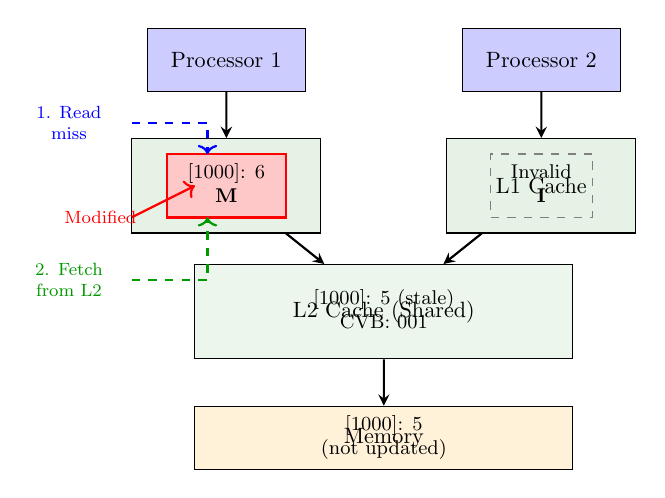
\begin{tikzpicture}[scale=0.8, transform shape]
% Define colors
\definecolor{cachecolor}{rgb}{0.9, 0.95, 0.9}
\definecolor{memcolor}{rgb}{1.0, 0.95, 0.85}

% Define styles
\tikzstyle{processor} = [rectangle, draw, fill=blue!20, minimum width=2.5cm, minimum height=1cm]
\tikzstyle{cache} = [rectangle, draw, fill=cachecolor, minimum width=3cm, minimum height=1.5cm]
\tikzstyle{memory} = [rectangle, draw, fill=memcolor, minimum width=4cm, minimum height=1cm]
\tikzstyle{arrow} = [->, thick, >=stealth]

% Processors
\node[processor] (p1) at (0,4) {Processor 1};
\node[processor] (p2) at (5,4) {Processor 2};

% L1 Caches
\node[cache] (l1p1) at (0,2) {L1 Cache};
\node[cache] (l1p2) at (5,2) {L1 Cache};

% L2 Cache
\node[cache, minimum width=6cm, fill=cachecolor!70] (l2) at (2.5,0) {L2 Cache (Shared)};

% Memory
\node[memory, minimum width=6cm] (mem) at (2.5,-2) {Memory};

% Connections
\draw[arrow] (p1) -- (l1p1);
\draw[arrow] (p2) -- (l1p2);
\draw[arrow] (l1p1) -- (l2);
\draw[arrow] (l1p2) -- (l2);
\draw[arrow] (l2) -- (mem);

% Cache contents - shown after pause
\visible<3->{
    % P1 L1 content
    \node[draw=red, thick, fill=modifiedcolor, font=\small] at (0,2) {
        \begin{tabular}{c}
        [1000]: 6\\
        \textbf{M}
        \end{tabular}
    };
}

\visible<4->{
    % P2 L1 content
    \node[draw=gray, dashed, font=\small] at (5,2) {
        \begin{tabular}{c}
        Invalid\\
        \textbf{I}
        \end{tabular}
    };
}

\visible<5->{
    % L2 content with CVB
    \node[font=\small] at (2.5,0) {
        \begin{tabular}{c}
        [1000]: 5 (stale)\\
        CVB: 001
        \end{tabular}
    };
}

\visible<6->{
    % Memory content
    \node[font=\small] at (2.5,-2) {
        \begin{tabular}{c}
        [1000]: 5\\
        (not updated)
        \end{tabular}
    };
}

% Annotations
\visible<3->{
    \node[text=red, font=\footnotesize] at (-2,1.5) {Modified};
    \draw[->, red, thick] (-1.5,1.5) -- (-0.5,2);
}

\visible<7->{
    % Transaction flow arrows
    \node[text=blue, font=\footnotesize, align=center] at (-2.5,3) {1. Read\\miss};
    \draw[->, blue, thick, dashed] (-1.5,3) -- (-0.3,3) -- (-0.3,2.5);
    
    \node[text=green!60!black, font=\footnotesize, align=center] at (-2.5,0.5) {2. Fetch\\from L2};
    \draw[->, green!60!black, thick, dashed] (-1.5,0.5) -- (-0.3,0.5) -- (-0.3,1.5);
}

\end{tikzpicture}

\pause[8]
\vspace{0.5em}
\begin{tcolorbox}[colback=yellow!10, colframe=orange!50, fonttitle=\footnotesize]
\textbf{Key Point:} First write after read transitions from E→M locally (no bus transaction needed)
\end{tcolorbox}

\end{columns}
\end{frame}

%==========================================
\begin{frame}{Ring Interconnect}
\begin{center}
% Placeholder for ring interconnect diagram
\framebox[0.8\textwidth][c]{
\parbox{0.75\textwidth}{\centering
[Diagram: Ring Interconnect Architecture\\
Cores 0-3 with LLC slices\\
System Agent, Graphics, IMC, DMI, PCI Express\\
Connected in ring topology]
}}
\end{center}
\end{frame}

%==========================================
\begin{frame}{Ring Architecture Details}
\textbf{Ring Configuration:}
\begin{itemize}
\item 2 × 4 rings: Req / Data / Ack / Snoop
\item Packets always use the shortest path
\item Static Even/Odd polarity per station
\item Each ring switches polarity on each cycle
\end{itemize}

\vspace{1em}
\begin{block}{Key Mechanism}
A stop can only pull data from the direction (ring) that matches its polarity in the current cycle
\begin{itemize}
\item[$\Rightarrow$] Sender must ensure data can be pulled by receiver when it arrives
\end{itemize}
\end{block}

\textbf{Example Configuration:}
\begin{itemize}
\item 64B cache line (L1/L2/LLC)
\item 32B/cycle bus bandwidth
\item[$\Rightarrow$] Cache line transfers from LLC to L1 in two strokes
\end{itemize}
\end{frame}

%==========================================
\begin{frame}{Ring Example - Data Transfer}
\footnotesize
\textbf{Scenario:} Core 0, Core 1, and GFX issue data read requests

\vspace{0.5em}
\begin{center}
% Placeholder for ring timing diagram
\framebox[0.9\textwidth][c]{
\parbox{0.85\textwidth}{\centering
[Timing Diagram: Ring cycles 1-15\\
Shows Request, Global Observation, and Data phases\\
Even/Odd polarity switching per cycle]
}}
\end{center}

\vspace{0.5em}
\textbf{Key Events:}
\begin{enumerate}
\item GFX request delayed (odd distance, must arrive on Even cycle)
\item Both Core requests hit in LLC, CVBs indicate no snoop needed
\item LLC sends first chunk (1/2 cache line) to each core
\item LLC sends GO with MESI state (E/S)
\item LLC sends second chunk to complete transfer
\end{enumerate}
\end{frame}

%==========================================
\begin{frame}{Summary}
\begin{itemize}
\item \textbf{MESI Protocol} ensures cache coherence in multi-processor systems
\vspace{0.5em}
\item \textbf{Four States:} Invalid, Shared, Exclusive, Modified
\vspace{0.5em}
\item \textbf{Key Mechanisms:}
    \begin{itemize}
    \item Core Valid Bits (CVB) for tracking
    \item Read For Ownership (RFO) for write intent
    \item Global Observation (GO) for state notification
    \end{itemize}
\vspace{0.5em}
\item \textbf{Ring Interconnect:} Efficient on-chip communication with polarity-based routing
\vspace{0.5em}
\item \textbf{Performance:} Message latencies crucial for overall system performance
\end{itemize}
\end{frame}

\end{document}